%\documentclass[notes,10pt,aspectratio=169]{beamer}

%\documentclass[notes, 10pt,aspectratio=169]{beamer}
\documentclass[10pt,aspectratio=169]{beamer}


% Add this line to your preamble
\setbeameroption{show notes on second screen=right}

%\usetheme{Singapore} %Boadilla, Madrid, default, etc. 
\usetheme[progressbar=frametitle]{metropolis}
\usecolortheme{rose} %beaver, dolphin, crane, 


%\setbeamersize{text margin left=4mm, text margin right=4mm}


\usecolortheme{default}

\usepackage[utf8]{inputenc}
\usepackage[T1]{fontenc}
\usepackage{lmodern}
\usepackage{xcolor}
\usepackage{tikz}
\usepackage{booktabs} % Required for \toprule, \midrule, \bottomrule
\usetikzlibrary{shapes.geometric, arrows, positioning}

\tikzstyle{block} = [rectangle, draw, text width=4cm, align=center, rounded corners, minimum height=1cm]
\tikzstyle{decision} = [rectangle, draw, text width=5cm, align=center, fill=blue!10, rounded corners, minimum height=1cm]
\tikzstyle{terminal} = [rectangle, draw, text width=4.5cm, align=center, fill=yellow!30, rounded corners, minimum height=1cm]
\tikzstyle{end} = [rectangle, draw, text width=5cm, align=center, fill=green!30, rounded corners, minimum height=1cm]
\tikzstyle{arrow} = [->, thick]



\usepackage{adjustbox}
%2. change the bullets 
\setbeamertemplate{itemize item}[triangle] %circle, square,... 


% 1. Define custom colors and set colors 
%\definecolor{myblue}{HTML}{003366}
\definecolor{accent}{RGB}{78,205,196}

%\setbeamercolor{title}{fg=white,bg=myblue}
\setbeamercolor{frametitle}{fg=black,bg=white}
%\setbeamercolor{normal text}{fg=mygray}
\setbeamercolor{block title}{fg=black,bg=blue}
%\setbeamercolor{block body}{fg=black,bg=white}

\setbeamercolor{item}{fg= orange!80} % Change bullet color
\setbeamercolor{button}{bg=orange, fg=white}



\AtBeginSection[]
{
  \begin{frame}{Outline}
    \tableofcontents[currentsection]%,hideothersubsections]
  \end{frame}
}

% 3. BibLaTeX settings
\usepackage[
  backend=biber,
  style=apa,
  citestyle=authoryear
]{biblatex}
\addbibresource{../references.bib}

\title{Equiilibrium effects of price updating: evidence from a centralized marketplace for annuities}
%\subtitle{A Mini Literature Overview}

\author{%
 Lucas Condeza
\inst{1} \and
   %\and
%  Coauthor Three\inst{3}
}
\institute{
  \inst{1} Yale University \\
}

\date{\today}

\begin{document}

\begin{frame}
  \titlepage
\end{frame}



 %%%%%%%%% Slide 2  %%%%%%%%%%%%%

\begin{frame}{Motivation} 
\begin{itemize}
    \item  In several markets consumers receive initial offers, then they can request revised offers. Examples: 
    \begin{itemize}
        \item Loans: consumers get a loan estimate (LE) and showing a LE to another lender could lead to a revised offer. [\href{https://chatgpt.com/share/68eaf593-1518-800d-b874-1fba1adbe177}{1}]
        \item Auto dealerships: buyers can shop around and dealers are willing to revise their initial offers [\href{https://chatgpt.com/share/68eaf593-1518-800d-b874-1fba1adbe177}{2}]
    \end{itemize}

    \item What are the impacts of allowing consumers to request revised offers?
    \item Economic forces at play: 
    \begin{itemize}
        \item Learning: firms learn competitors' prices and can best respond.
        \item Discrimination: if search cost are correlated with preferences. [not today] 
    \end{itemize}
\end{itemize}
\note{
    \begin{itemize}
        \item I am going to study the effects of being able to request revised offers in a centralized marketplace for annuities in Chile.  
    \end{itemize}}
\end{frame}

%%%%%%%%% Slide 3 %%%%%%%%%%%%%

\begin{frame}{This research}
\begin{itemize}
    \item Studies a centralized marketplace for annuities in Chile (SCOMP)
    \item A recent law eliminated the possibility of requesting revised offers.
    \begin{itemize}
        \item Before: consumers receive initial offers, then can request revised offers from one firm.
        \item After: consumers can only accept/reject initial offers.
        \item Rationale for elimination: "firms will not make their best efforts in the initial phase"
    \end{itemize}
    \item Also provides evidence on assymmetries in infomration precision in selection markets. 
\end{itemize}
\end{frame}

 %%%%%%%%% Slide 4 %%%%%%%%%%%%%

\begin{frame}{Literature}


\begin{itemize}
    \item Search in selection markets: \textcite{allen_search_2019} %larsen_efficiency_2021


    \item Competition in selection markets: \textcite{mahoney_imperfect_2017, cuesta_price_2018, cosconati_competing_2025} %Crawford et al 2018

    \item Centralized marketplaces in selection markets : %Tebaldi (2024), 
    
    \item SCOMP specific: % boehm 2024, illanes and padi 2019, alcalde and via.  % 
    
    %\item Selection in multiple dimensions: \textcite{finkelstein_adverse_2004} and Finkelstein and McGarry (2006).  

    %\item Aftermarkets: \textcite{allen_search_2019} %larsen_efficiency_2021
     
\end{itemize}
\note{
\textcolor{blue}{ ADD THE CONTRIBUTIONS TO EACH LITERATURE AND ADD MORE PAPERS}
}
\end{frame}

%%%%%%%%%

\section{Setting and Data}

%%%%%%%%% Slide 6 %%%%%%%%%%%%%
\begin{frame}{Setting: annuities}\label{slide:setting}
    
    \begin{itemize}%[<+->]
    \item Annuities: transform a stock of savings into a stream of payments until death.
    \item Reasons to buy: insure against overlife risk
        \item Profits of firm $j$: 
    \begin{align*}
    \pi_{ji}(F) = S_i-  \mathbb{E}^j_{T} \left[\sum_{t=1}^T\frac{F}{(1+r_j)^t}|x_i \right]
    \end{align*}
    % if it was only financing cost, it would be a monopoly
   
     $S$: stock of savings, $F$: per period annuity payment, $x_i$: individual mortality factors
    
    \item Firm heterogeneity: algorithm (mortality tables), financing costs ($r_j$) and risk ratings. 
    
    \item Our setti
    \end{itemize}


    \note{
    \begin{itemize}
        \item Explicitly not link the annuities market with pensions because generates confusion
        \item Explain what annuities are. 
    \end{itemize}}
\end{frame}


\begin{frame}{SCOMP Process Flow Diagram}\label{slide:setting2}
\begin{center}
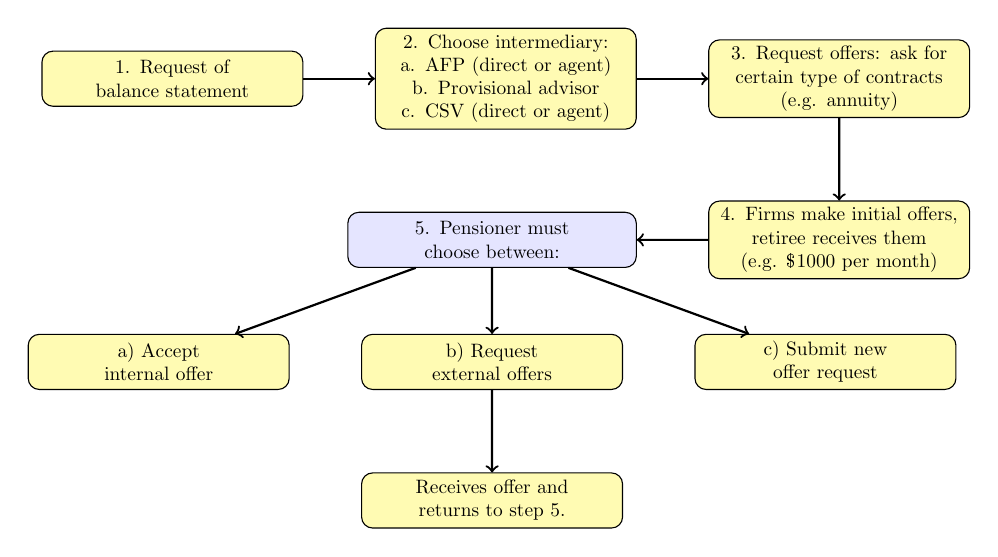
\begin{tikzpicture}[node distance=1.5cm and 1.3cm, scale=0.7, every node/.style={transform shape}]

\node[terminal] (step1) {1. Request of \\  balance statement};
\node[terminal, right=of step1] (step2) {2. Choose intermediary:\\a. AFP (direct or agent)\\b. Provisional advisor\\c. CSV (direct or agent)};
\node[terminal, right=of step2] (step3) {3. Request offers: ask for certain type of contracts \\ (e.g. annuity) };
\node[terminal, below =of step3] (step4) {4. Firms make initial offers, \\ retiree receives them (e.g. \$1000 per month)};

% **CHANGES MARKED**: Second row - right to left
\node[decision, left=of step4] (step5) {5. Pensioner must\\choose between:};


% **CHANGES MARKED**: Third row - decision and outcomes (left to right)
\node[terminal, below=1.2cm of step5] (choice_b) {b) Request\\external offers};
\node[terminal, left=of choice_b] (choice_a) {a) Accept\\internal offer};
\node[terminal, right= of choice_b ] (choice_c) {c) Submit new\\offer request};

% Additional choices below decision
\node[terminal, below=of choice_b] (choice_b2) {Receives offer and returns to step 5.};
%\node[terminal, below=0.8cm of choice_b] (no_pension) {d) Not retire};


% **CHANGES MARKED**: Horizontal flow arrows - first row (left to right)
\draw[arrow] (step1) -- (step2);
\draw[arrow] (step2) -- (step3);
\draw[arrow] (step3) -- (step4);
\draw[arrow] (step4) -- (step5);

% **CHANGES MARKED**: Second row arrows (right to left)
\draw[arrow] (choice_b) -- (choice_b2);
\draw[arrow] (step5) -- (choice_a);
\draw[arrow] (step5) -- (choice_b);
\draw[arrow] (step5) -- (choice_c);

\end{tikzpicture}
\end{center}
\begin{itemize}
    \item \hyperlink{slide:fig_offer_certificate}{\beamerbutton{Offer Certificate}}
\end{itemize}
\end{frame}

%%%%%%%%%

\begin{frame}{Data} \label{slide:data}
\begin{itemize}
    \item SCOMP data at the individual level  
    \begin{itemize}
        \item Posted and revised prices, and consumer decisions 
        \item Total savings 
        \item Demographics: age and gender \hyperlink{slide:fig_offer_certificate}{\beamerbutton{Certificate with initial prices}}
    \end{itemize}
     \item Retirement insurance companies: risk ratings
\end{itemize}

Particularities of the data/setting: 

\begin{itemize}
    \item One observes all the offers received by the buyers 
    \item One observes the same information as the firms (gender, age, savings)
\end{itemize}
\end{frame}

%%%%%%%%%%%%%%%%%%%%%%%%%%%%%%%%%%%%%%%%%%%%%%%%%%%%%%

\section{Empirical Evidence}
 

\begin{frame}{Descriptive Evidence}\label{slide:Descriptive_evidence}
\begin{itemize}
    \item Most buyers request external offers and the improvement is sizeable. \hyperlink{slide:fig1}{\beamerbutton{External offers}} 
    \item Products are differentiated \hyperlink{slide:fig2}{\beamerbutton{Foregone value}} 
    \item Selection into companies \hyperlink{slide:fig3}{\beamerbutton{Heterogeneity in algorithm precision}}
    \item Firms learn about other firms' prices  \hyperlink{slide:fig4}{\beamerbutton{Learning}} 
\end{itemize}
\end{frame}


%%%%

\begin{frame}\frametitle{Prevalence of external offers}\label{slide:fig1}
\begin{figure}
    \centering
    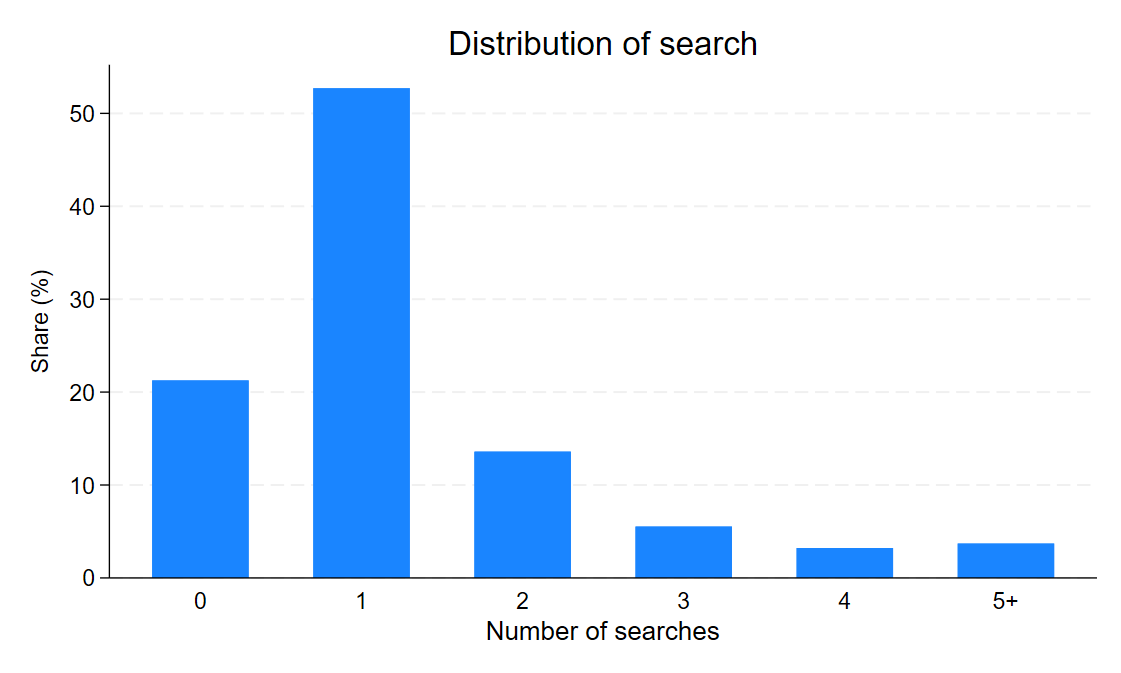
\includegraphics[width=0.49\textwidth]{../figures/IE3_dist_external_offers.png}
    \hfill 
    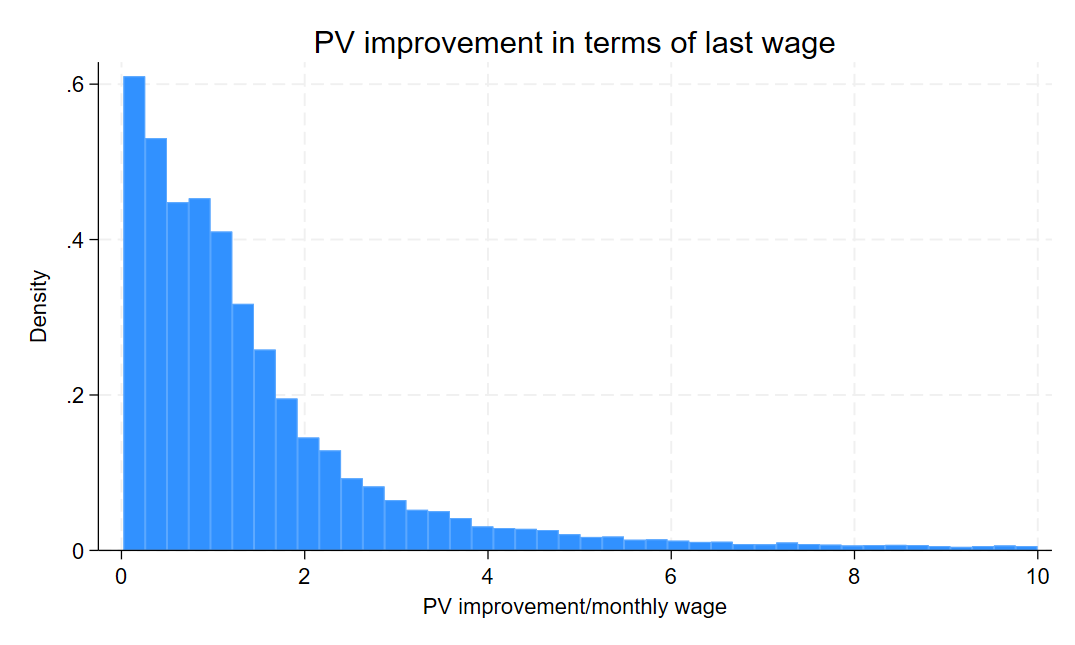
\includegraphics[width=0.49\textwidth]{../figures/IE3_offer_improvement_histogram.png}
\end{figure}

\begin{itemize}
    \item   75\% of the purchases are through external offers. 
     \hyperlink{slide:Descriptive_evidence}{\beamerbutton{Go back}}   
\end{itemize}

\note{
That only some people use the aftermarket suggest: 
\begin{itemize}
    \item There are search costs 
    \item Firms could be discriminating based on the search likelihood. 
\end{itemize}
Any assessment of the welfare effects of the aftermarket has to consider that by banning it buyers will save in search costs, but will not be able to improve on the initial posted prices. 

In a model where search costs are not correlated with valuations, the aftermarket prices by the sellers are the same as the initial prices.
}
\end{frame}

%%%%%%%%%%%%%%%%%%%%%%%%%%%%%%%%%%%%%%%%%%%%%%%%%%%%%%

\begin{frame}{Differentiation}\label{slide:fig2}    
Buyers do not always buy highest annuity. Average foregone value is 1.57 monthly wages.
\begin{figure}[H]
%\caption{}
\centering{}%
\begin{tabular}{cc}
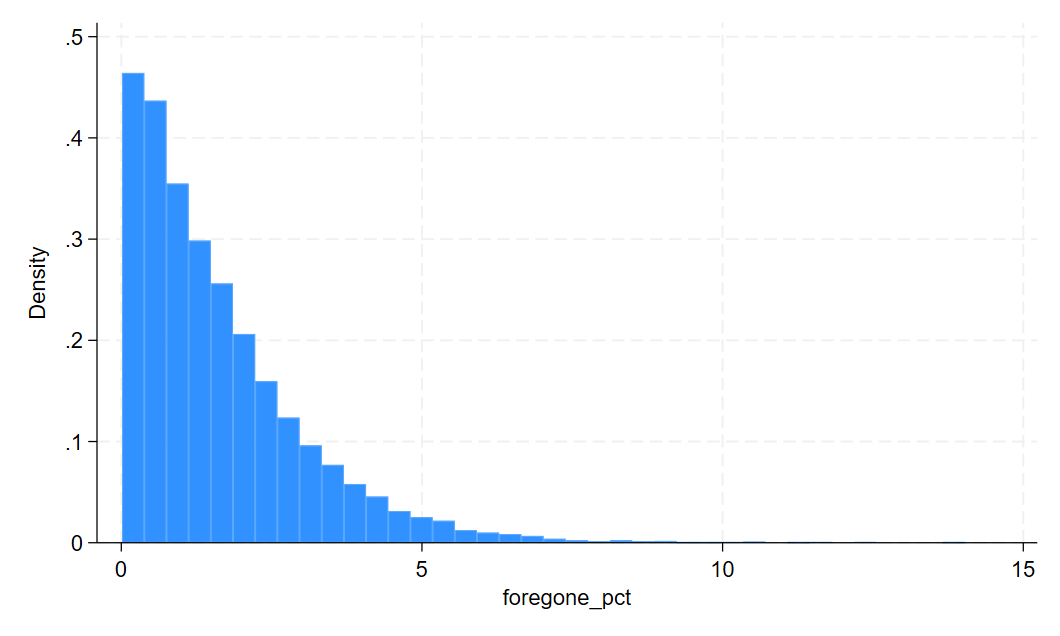
\includegraphics[scale=0.25]{../figures/IE3_foregone_hist.png}
\end{tabular}
\end{figure}
\hyperlink{slide:Descriptive_evidence}{\beamerbutton{Go back}}
\end{frame}

%%%%%%%%%%%%%%%%%%%%%%%%%%%


\begin{frame}{Heterogeneity in algorithm precision}\label{slide:fig3}    
\begin{figure}[H]
%\caption{}
\centering{}%
\begin{tabular}{cc}
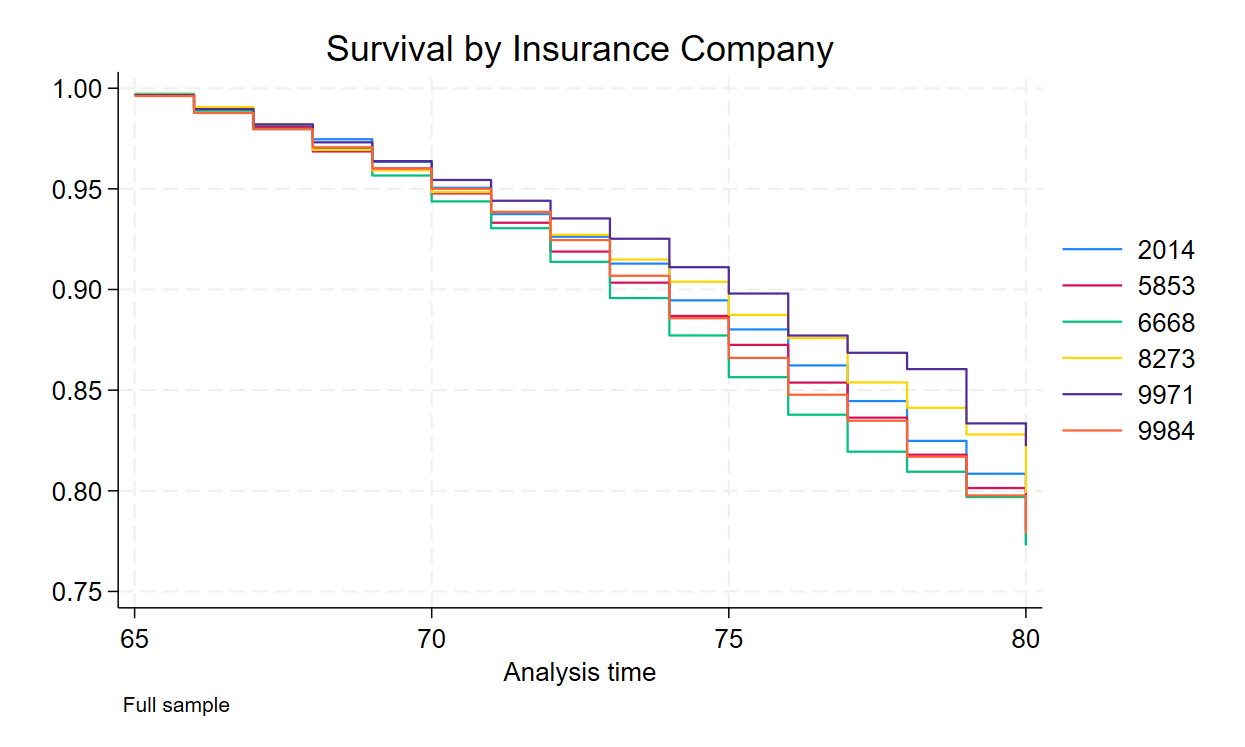
\includegraphics[scale=0.264]{../figures/IE6/IE6_survival_year_all.png}
\end{tabular}
\end{figure}
\hyperlink{slide:Descriptive_evidence}{\beamerbutton{Go back}}
\end{frame}


\begin{frame}{Learning}\label{slide:fig4}    
\scalebox{0.8}{
    {
\def\sym#1{\ifmmode^{#1}\else\(^{#1}\)\fi}
\begin{tabular}{l*{7}{c}}
\hline\hline
                    &\multicolumn{1}{c}{(1)}&\multicolumn{1}{c}{(2)}&\multicolumn{1}{c}{(3)}&\multicolumn{1}{c}{(4)}&\multicolumn{1}{c}{(5)}&\multicolumn{1}{c}{(6)}&\multicolumn{1}{c}{(7)}\\
                    &\multicolumn{1}{c}{Increase}&\multicolumn{1}{c}{Increase}&\multicolumn{1}{c}{Increase}&\multicolumn{1}{c}{Increase}&\multicolumn{1}{c}{Increase}&\multicolumn{1}{c}{Increase}&\multicolumn{1}{c}{Has External Offer}\\
\hline
main                &                     &                     &                     &                     &                     &                     &                     \\
Avg. Gap            &       0.316\sym{***}&       0.155\sym{***}&       0.155\sym{***}&       0.139\sym{***}&       0.147\sym{***}&       0.071\sym{***}&                     \\
                    &     (0.006)         &     (0.010)         &     (0.010)         &     (0.016)         &     (0.019)         &     (0.020)         &                     \\
[1em]
Max. Gap            &                     &       0.110\sym{***}&       0.110\sym{***}&                     &      -0.021         &      -0.006         &                     \\
                    &                     &     (0.009)         &     (0.009)         &                     &     (0.029)         &     (0.028)         &                     \\
[1em]
gap\_from\_avg        &                     &                     &                     &                     &                     &                     &      -0.191\sym{***}\\
                    &                     &                     &                     &                     &                     &                     &     (0.032)         \\
[1em]
Constant            &       1.893\sym{***}&       1.375\sym{***}&       1.375\sym{***}&       1.381\sym{***}&       1.387\sym{***}&       1.511\sym{***}&      -2.012\sym{***}\\
                    &     (0.010)         &     (0.082)         &     (0.082)         &     (0.045)         &     (0.046)         &     (0.121)         &     (0.028)         \\
\hline
Observations        &       14133         &       14133         &       14133         &        2046         &        2046         &        2046         &       16164         \\
\hline\hline
\multicolumn{8}{l}{\footnotesize Average: is the difference between the mean of other firms' initial offers and own initial offer}\\
\multicolumn{8}{l}{\footnotesize Max Gap: is the difference between the highest other firm's initial offer and own initial offer.}\\
\multicolumn{8}{l}{\footnotesize Cols (1)-(3) use the population of initial offers that are not the highest, (4)-(6) only use the highest offer}\\
\multicolumn{8}{l}{\footnotesize Cols (4) and (6) include firm fixed effects}\\
\end{tabular}
}

}
\hyperlink{slide:Descriptive_evidence}{\beamerbutton{Go back}}
\end{frame}


\begin{frame}{Learning(1)}\label{slide:fig5}
  \begin{figure}[H]
%\caption{}
\centering{}%
\begin{tabular}{cc}
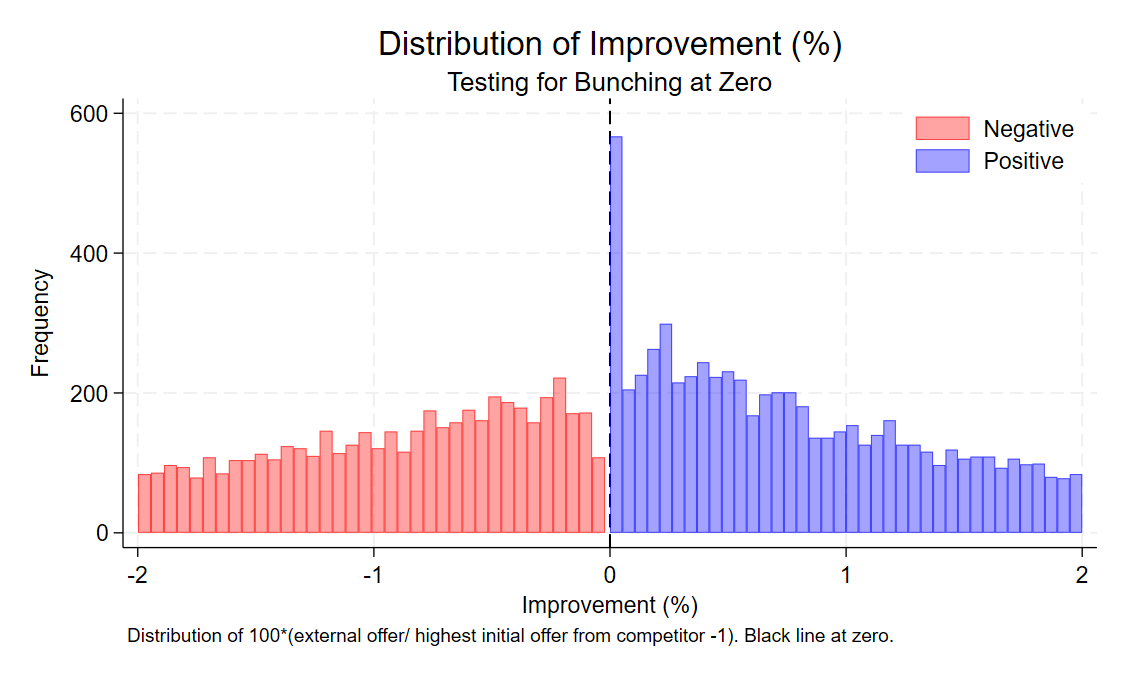
\includegraphics[scale=0.39]{../figures/IE7/IE7_hist_bunching_max(2).png} 
\end{tabular}
\end{figure}
\hyperlink{slide:Descriptive_evidence}{\beamerbutton{Go back}}
\end{frame}


%%%%%%%%%%%%%%%%%%%%%%%%%%%%%%%%%%%%%%%%%%%%%%%%%%%%%%%%%%%%%%%%%%%%%%%%%%%%%%%%
\section{Model and Simulations}


\begin{frame}{Learning Model: Overview}
\begin{itemize}
    \item \textbf{Goal:} Rationalize the increase in offers between initial and external offers
    
    \item \textbf{Key mechanism:} Firms learn competitors' offers when consumer requests external offers
    
    \item \textbf{Setup:}
    \begin{itemize}
        \item One consumer and $J$ firms
        \item Firm $j$ has private cost $c_j \sim F_j$ (due to interest rate variation)
        \item Consumer chooses firm with probability $D_j(p)$ (logit demand)
    \end{itemize}
    
    \item \textbf{Innovation:} Two-stage pricing with learning opportunity
\end{itemize}
\end{frame}

%%%%%

\begin{frame}{Two-Stage Game: Timeline}
\begin{enumerate}
    \item \textbf{Stage 1 (Initial offers):}
    \begin{itemize}
        \item Firms simultaneously post initial prices $p^{T1}_j$
        \item Consumer observes all offers
    \end{itemize}
    
    \vspace{0.3cm}
    
    \item \textbf{Consumer decision:}
    \begin{itemize}
        \item With probability $1-\lambda$: accepts one of the initial offers
        \item With probability $\lambda$: requests external offer from random firm
    \end{itemize}
    
    \vspace{0.3cm}
    
    \item \textbf{Stage 2 (External offers):}
    \begin{itemize}
        \item Selected firm observes all initial offers $p^{T1}$
        \item Can update its offer: $p^{T2}_j(c_j, p^{T1}) = \min(p^{T1}_j, p^*)$
        \item Consumer chooses among all available offers
    \end{itemize}
\end{enumerate}
\end{frame}

%%%%%

\begin{frame}{Second Stage: Optimal Pricing with Learning}
\textbf{When selected for external offer, firm observes competitors' initial prices}

\vspace{0.3cm}

\textbf{Optimal updated offer:}
$$p^{T2}_j(c_j, p^{T1}) = \min(p^{T1}_j, p^*)$$

where
$$p^* = \arg\max_{p_j} (p_j - c_j) D_j(p_j, p^{T1}_{-j})$$

\vspace{0.5cm}

\textbf{Key insight:} Firm can only lower its price (or keep it unchanged)

\vspace{0.3cm}
After observing competitors, firm best-responds to known prices rather than expected prices
\end{frame}

%%%%%

\begin{frame}{Expected Profits in Second Stage}
\textbf{When consumer searches, firm $j$ faces two scenarios:}

\vspace{0.3cm}

\textbf{1. Selected for external offer ($\frac{1}{J}$ probability):}
$$\pi^{(j)}_j(p^{T1}, c_j) = (p^{T2}_j(c_j, p^{T1}) - c_j) D_j(p^{T2}_j(c_j, p^{T1}), p^{T1}_{-j})$$

\vspace{0.3cm}

\textbf{2. Competitor $j'$ selected ($\frac{1}{J}$ probability):}
$$\pi^{(j')}_j(p^{T1}, c_j, c_{j'}) = (p^{T1}_j - c_j) D_j(p^{T1}_{-j'}, p^{T2}_{j'}(c_{j'}, p^{T1}))$$

\vspace{0.5cm}

\textbf{Expected second stage profits:}
$$\pi^{T2}_j(p^{T1}, c_j, c_{-j}) = \frac{1}{J}\left[\pi^{(j)}_j(p^{T1}, c_j) + \sum_{j' \neq j} \pi^{(j')}_j(p^{T1}, c_j, c_{j'})\right]$$
\end{frame}

%%%%%

\begin{frame}{First Stage: Strategic Pricing}
\textbf{Firms anticipate the second stage when setting initial prices}

\vspace{0.5cm}

\textbf{Expected profits in first stage:}
$$\pi^{T1}_j(p^{T1}, c_j, c_{-j}) = (1-\lambda)\underbrace{(p^{T1}_j - c_j)D_j(p^{T1})}_{\text{Immediate acceptance}} + \lambda \underbrace{\pi^{T2}_j(p^{T1}, c_j, c_{-j})}_{\text{Search occurs}}$$

\vspace{0.5cm}

\textbf{Equilibrium condition:}
$$p^{T1}_j(c_j) = \arg\max_{p_j} \int \pi^{T1}_j(p_j, p^{T1}_{-j}(c_{-j}), c_j) dF(c_{-j}|c_j)$$

\vspace{0.3cm}
Trade-off: higher initial price (if accepted) vs. competitive position if search occurs
\end{frame}


\begin{frame}{Simulations }
\begin{figure}[H]
\centering{}%
\begin{tabular}{cc}
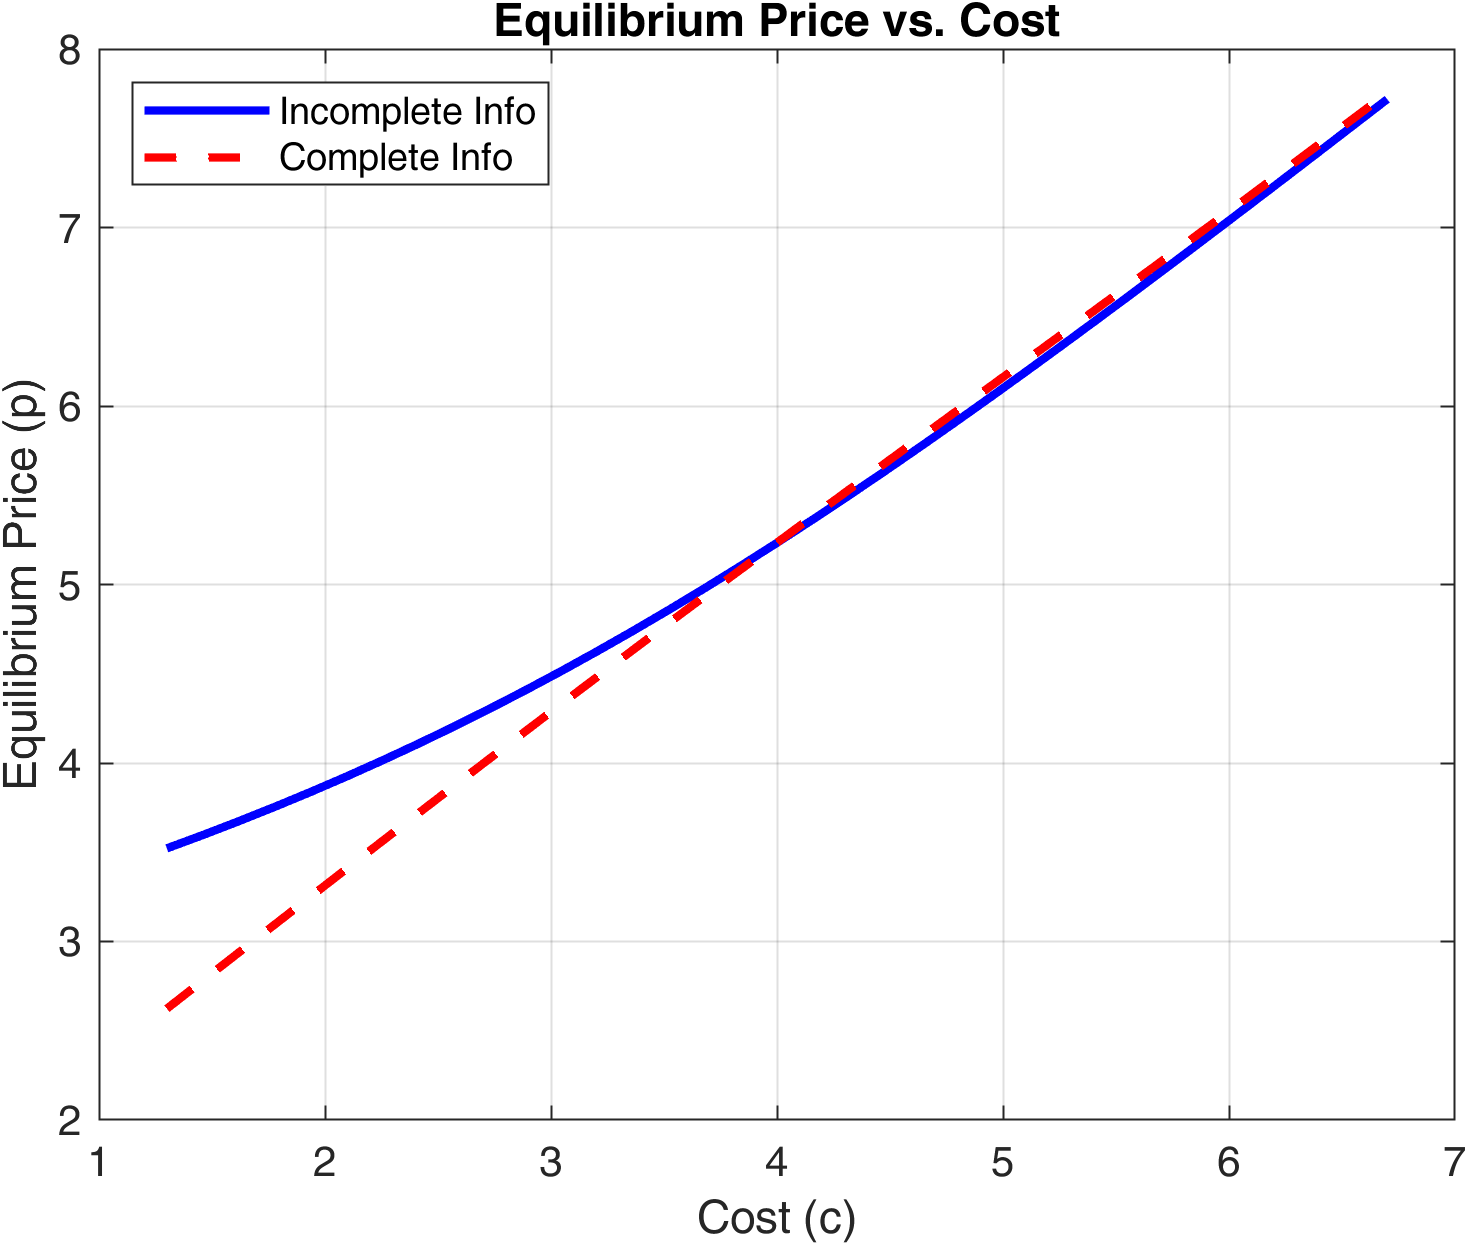
\includegraphics[scale=0.7]{../figures/simulations/model5/pricesCI_IC.png}
\end{tabular}
\end{figure}
\end{frame}



\begin{frame}{Initial prices}\label{slide:fig_offer_certificate}    
\begin{figure}[H]
\centering{}%
\begin{tabular}{cc}
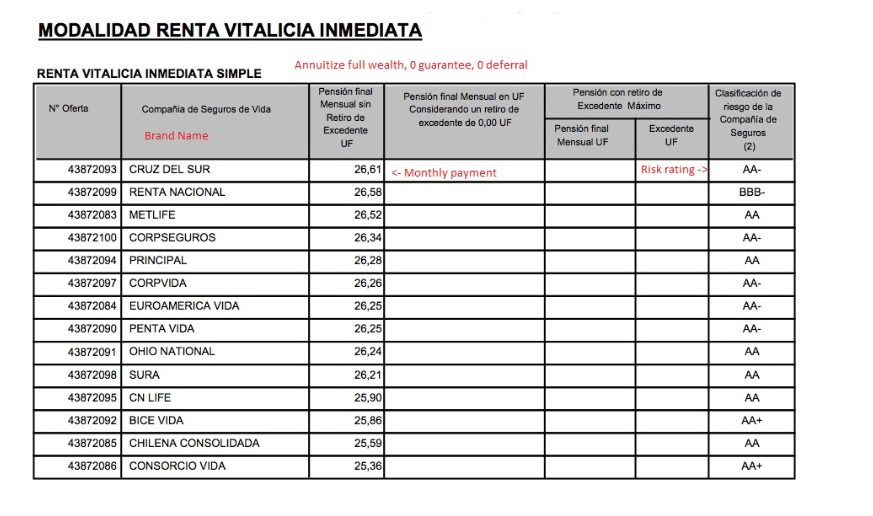
\includegraphics[scale=0.49]{../figures/annuity_offer.png}
\end{tabular}
\end{figure}
\hyperlink{slide:setting2}{\beamerbutton{Go back: Diagram}} 
\hyperlink{slide:data}{\beamerbutton{Go back: Data}}
\end{frame}



\end{document}